% ============================================================================
% DOE Office of Science, FY 2027 open call, NOFO DE-FOA-0003665
% Pre-application ("also called white paper", Part 1 p. 105) to
% Basic Energy Sciences, Materials Sciences and Engineering Division,
% Synthesis and Processing Science (Part 1 pp. 24-25; contact Shawn Chen).
% Target date for white papers or pre-applications: November 30, 2026.
% Submitted through DOE SC PAMS, not by email (Part 1 pp. 106-107;
% Part 2 pp. 17-18).
%
% Format (Part 1 p. 106): title page first, not counted; then at most three
% pages on letter paper, 1 in margins, body text at least 11 pt; figures and
% references must fit within the three pages. The senior/key personnel list
% and the list of individuals who should not serve as merit reviewers go in
% a separate "Additional Attachment" in PAMS and do not count.
%
% Sources and open questions: README.md in this folder.
% Build: xelatex white-paper.tex (twice)
% ============================================================================

\documentclass[11pt,letterpaper]{article}

\usepackage[margin=1in]{geometry}
\usepackage{iftex}
\ifPDFTeX
  \usepackage[T1]{fontenc}
  \usepackage[utf8]{inputenc}
  \usepackage{mathptmx}
\else
  \usepackage{fontspec}
  \IfFontExistsTF{Times New Roman}
    {\setmainfont{Times New Roman}}
    {\setmainfont{TeX Gyre Termes}}
\fi
\usepackage{microtype}
\usepackage{flafter}  % floats never appear before their place in the text
\usepackage{array}
\usepackage{tikz}
\usetikzlibrary{arrows.meta}
\usepackage[font=normalsize,labelfont=bf,labelsep=period,skip=3pt]{caption}
\usepackage[colorlinks=true,linkcolor=blue!60!black,citecolor=blue!60!black,
  urlcolor=blue!60!black]{hyperref}
\usepackage{titlesec}
\titleformat{\section}{\normalfont\normalsize\bfseries}{\thesection.}{0.5em}{}
\titlespacing*{\section}{0pt}{6pt plus 2pt minus 1pt}{2pt}

\setlength{\parindent}{0pt}
\setlength{\parskip}{4pt plus 1pt minus 1pt}
\setlength{\textfloatsep}{8pt plus 2pt minus 2pt}
\pagestyle{plain}

\begin{document}

% ===========================================================================
% Title page (does not count toward the three-page limit; Part 1 p. 106)
% ===========================================================================
\thispagestyle{empty}
\begin{center}
{\Large\bfseries Nucleation, Freezing Range, and Hot Cracking\\
in Aluminum Alloys Solidified at Laser Melting Rates\par}
\vspace{14pt}
Sterling G.\ Baird, Ph.D., Assistant Professor, Department of Mechanical
Engineering\\
Brigham Young University (lead institution), Provo, UT 84602\\
(801) 422-5344, \href{mailto:sterling.baird@byu.edu}{sterling.baird@byu.edu}\\
NOFO Number: DE-FOA-0003665
\end{center}
\vspace{12pt}
\begin{tabular}{@{}>{\bfseries}p{1.8in}>{\raggedright\arraybackslash}p{4.5in}@{}}
Senior/key personnel & Sterling G.\ Baird (PI), Brigham Young University.
  No other senior/key personnel and no team member institutions. \\[4pt]
Research area & Basic Energy Sciences, Materials Sciences and Engineering
  Division, Synthesis and Processing Science (NOFO Part 1, Section III) \\[4pt]
Program manager & Shawn Chen \\
\end{tabular}

\clearpage
\setcounter{page}{1}

% ===========================================================================
% Pre-application body (three-page limit, figures and references included)
% ===========================================================================
\section{Scientific questions}

Most high-strength aluminum alloys, such as 7075, are unsuitable for laser
powder bed fusion (LPBF): printing gives large columnar grains and periodic
cracks~\cite{martin2017}. Martin et al.\ removed both by assembling
zirconium-based nanoparticles onto the powder, which gave crack-free,
equiaxed, fine-grained material~\cite{martin2017}. That result leaves the
mechanism open. We ask three questions.
(1) Why does a given addition of zirconium or scandium give equiaxed grains
under some laser conditions and columnar grains under others?
(2) Why does cracking follow the shape of the solidification curve near its
end~\cite{kou2015}, and how do grain shape and the loss of magnesium and zinc
by evaporation~\cite{debroy2018} change that relation?
(3) How far do equilibrium and Scheil calculations of phase diagrams (CALPHAD)
depart from what actually forms when aluminum solidifies at LPBF speeds?

The laser is a moving, localized heat source. The thermal gradient $G$ and
solidification speed $R$ it imposes at the back of the melt pool direct how
grains grow, and both change with laser power and scan speed. A single build
plate can therefore hold dozens of single tracks, each solidified under
different conditions that we can estimate. These questions concern nucleation and phase
transitions far from equilibrium, and the answers apply to welding and other
rapid solidification processes as well as to printing.

\section{Hypotheses and tests}

\textbf{H1, nucleation.} Equiaxed grains form only if primary
Al$_3$Zr or Al$_3$(Sc,Zr) particles precipitate in the cooling liquid before
the aluminum grows past them. At higher scan speed the liquid spends less
time in that window, so fewer particles act as nucleants. Prediction: the
smallest Zr\,+\,Sc content that gives equiaxed grains rises with scan speed,
and the boundary follows Hunt's criterion for the columnar-to-equiaxed
transition~\cite{hunt1984}, with the nucleant density computed from the
CALPHAD primary-particle fraction. H1 is rejected if that critical content
does not change with scan speed beyond the scatter of replicate tracks.

\textbf{H2, cracking.} Crack density at LPBF speeds is set by Kou's index,
the steepness of temperature against the square root of fraction solid near
the end of solidification~\cite{kou2015}, when the index is computed for the
composition that actually solidifies, after evaporation. Equiaxed grains raise
the index at which cracks first appear. Prediction: crack density against the
index falls on two separate curves, one for columnar and one for equiaxed
tracks, and the measured composition ranks cracking better than the nominal
one. H2 is rejected if neither grain shape nor the composition correction
improves the rank correlation between index and crack density.

\textbf{H3, departure from CALPHAD.} At LPBF solidification speeds the
growing solid traps solute and some intermetallic phases do not form.
Prediction: measured freezing behavior and phase fractions lie between
equilibrium and Scheil predictions at low scan speed and move outside the
Scheil bound as speed rises. H3 is rejected if measured phase fractions and
segregation stay within the Scheil bound at every speed tested.


\begin{figure}[t]
\centering
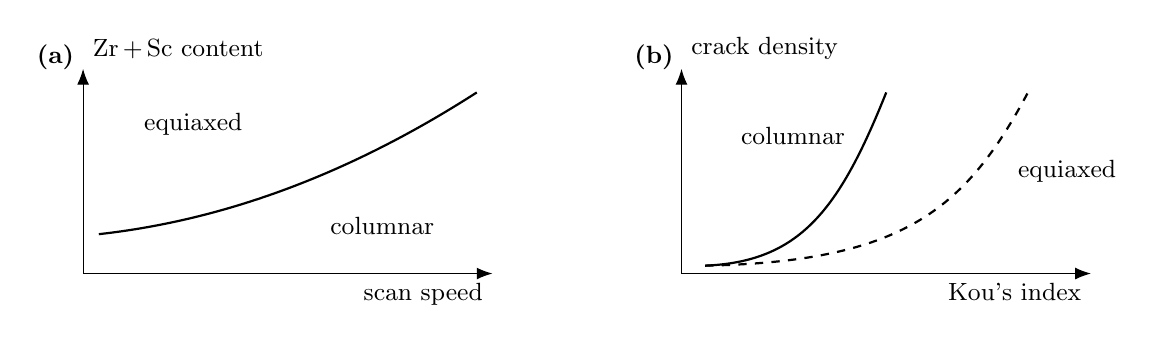
\begin{tikzpicture}[font=\small, >={Latex[length=2mm]}]
  % Panel (a): H1
  \draw[->] (0,0) -- (5.2,0) node[below left, align=right] {scan speed};
  \draw[->] (0,0) -- (0,2.6) node[above right] {Zr\,+\,Sc content};
  \draw[thick] (0.2,0.5) .. controls (2.0,0.7) and (3.6,1.4) .. (5.0,2.3);
  \node at (1.4,1.9) {equiaxed};
  \node at (3.8,0.6) {columnar};
  \node[font=\small\bfseries] at (-0.35,2.75) {(a)};
  % Panel (b): H2
  \begin{scope}[xshift=7.6cm]
  \draw[->] (0,0) -- (5.2,0) node[below left] {Kou's index};
  \draw[->] (0,0) -- (0,2.6) node[above right] {crack density};
  \draw[thick] (0.3,0.1) .. controls (1.5,0.15) and (2.0,0.8) .. (2.6,2.3);
  \draw[thick, dashed] (0.3,0.1) .. controls (2.8,0.15) and (3.6,0.8) .. (4.4,2.3);
  \node[anchor=east] at (2.2,1.75) {columnar};
  \node[anchor=west] at (4.15,1.3) {equiaxed};
  \node[font=\small\bfseries] at (-0.35,2.75) {(b)};
  \end{scope}
\end{tikzpicture}
\caption{Sketched predictions. (a) H1: the nucleant content needed for
equiaxed grains rises with scan speed. (b) H2:
equiaxed tracks crack at a higher index than columnar tracks of the same
alloy.}
\label{fig:predictions}
\end{figure}

\section{Approach}

\textbf{Alloys and powder.} We will study an Al-Zn-Mg-Cu base near 7075 with
zirconium and scandium additions over a range of contents. Powder for each
composition is made in our laboratory by an ultrasonic atomizer (AMAZEMET
rePOWDER) with an induction-melting module, at four compositions per week.
Making our own powder lets us change composition in small steps each
week.

\textbf{Controlled solidification.} LPBF builds are bought on a purchase
order from a University of Utah user facility at \$800 per build. Each plate
holds single tracks over a grid of laser power and scan speed, plus small
cubes at selected settings, with replicates to measure scatter. We will
estimate $G$ and $R$ for each track from its melt-pool cross-section and scan
speed, calibrated with a thermal model.

\textbf{Measurements.} At the BYU Microscopy Center, scanning electron
microscopy (SEM) gives melt-pool shape and crack density, electron
backscatter diffraction (EBSD) gives grain shape and the equiaxed fraction,
and energy-dispersive X-ray spectroscopy (EDS) gives magnesium and zinc loss
and solute segregation across cells. Tensile and hardness tests on selected
compositions connect grain shape to strength and ductility.

\textbf{Calculations.} Equilibrium and Scheil CALPHAD calculations run on BYU
high-performance computing for every composition, on both the nominal and the
measured composition. They supply the primary-particle fraction and formation
temperature (H1), Kou's index (H2), and the reference phase fractions that H3
tests.

\textbf{Choosing experiments.} The composition and laser space is too large
to measure on a grid, and the measurements differ in cost from minutes
(calculations) to days (tensile tests). Statistical models linked in the same
order as the steps~\cite{astudillo2021} let us choose the next compositions
and laser settings where H1 to H3 and their alternatives predict the most
different outcomes per unit cost. Each composition then stops at the cheapest
measurement that answers the question~\cite{buathong2024}: most stop at
tracks, and few reach tensile tests. We are extending this method to several
outputs at once and to results that arrive at different times. In this
project its role is to place experiments near the transitions in H1 and H2.

\textbf{Alternatives.} Nucleant particles may survive from the powder
instead of forming in the melt pool. A second laser pass over the same
track separates the two: particles carried over from the powder are lost on
remelting, while particles that form in the cooling liquid form again. If
cracking does not follow Kou's index at all, we will compare crack density
with the CALPHAD freezing range and with the fraction of liquid left at the
end of solidification, which are older measures of cracking tendency.

\textbf{Plan.} Year~1 tests H3 and H1 on tracks for zirconium-only alloys
over a range of scan speeds, including remelting tests. Year~2 adds scandium
and zirconium plus scandium, builds cubes, and tests H2. Year~3 tests the
combined rule on new compositions chosen to challenge it, adds tensile tests,
and releases the data.

\section{Expected results and team}

The project will produce measured maps of grain shape and cracking across
composition, $G$, and $R$ for Al-Zn-Mg-Cu alloys with Zr and Sc. It will also
give a tested rule for when a nucleant addition gives equiaxed grains at high
solidification speed, measured departures from equilibrium and Scheil
predictions at LPBF speeds, and open data and code. Results that reject a
hypothesis will be published like any other.

Since the laboratory opened at Brigham Young University (BYU) in December
2025, we have set up the CALPHAD workflow on BYU high-performance computing
and completed a powder-to-part demonstration on a baseline aluminum alloy:
atomized powder, LPBF builds, SEM and EDS, and tensile data. In a hand-built,
noise-free simulation in which a CALPHAD crack screen ignored zirconium,
choosing each next measurement by expected gain per cost matched the best
result of screening first after 3.8 times less spending (90\% confidence
interval 2.0 to 5.7). The PI (Ph.D., Materials Science and Engineering,
University of Utah, 2023) inferred grain boundary models with propagated
uncertainty, developed Honegumi for setting up Bayesian optimization, and
co-authored the \emph{Chemical Reviews} survey of self-driving laboratories.
The PI will supervise one Ph.D.\ student and two part-time undergraduate
researchers over three years.

\renewcommand{\refname}{References}
\begingroup
\setlength{\itemsep}{0pt}
\raggedright
\begin{thebibliography}{9}
\setlength{\itemsep}{1pt}
\setlength{\parskip}{0pt}

\bibitem{martin2017}
J.\,H. Martin et al., ``3D printing of high-strength aluminium alloys,''
\emph{Nature} \textbf{549}, 365-369 (2017).
\href{https://doi.org/10.1038/nature23894}{doi:10.1038/nature23894}

\bibitem{kou2015}
S.~Kou, ``A criterion for cracking during solidification,'' \emph{Acta
Mater.} \textbf{88}, 366-374 (2015).
\href{https://doi.org/10.1016/j.actamat.2015.01.034}{doi:10.1016/j.actamat.2015.01.034}

\bibitem{debroy2018}
T.~DebRoy et al., ``Additive manufacturing of metallic components: Process,
structure and properties,'' \emph{Prog. Mater. Sci.} \textbf{92}, 112-224
(2018).
\href{https://doi.org/10.1016/j.pmatsci.2017.10.001}{doi:10.1016/j.pmatsci.2017.10.001}

\bibitem{hunt1984}
J.\,D. Hunt, ``Steady state columnar and equiaxed growth of dendrites and
eutectic,'' \emph{Mater. Sci. Eng.} \textbf{65}, 75-83 (1984).
\href{https://doi.org/10.1016/0025-5416(84)90201-5}{doi:10.1016/0025-5416(84)90201-5}

\bibitem{astudillo2021}
R.~Astudillo and P.\,I. Frazier, ``Bayesian optimization of function
networks,'' \emph{Adv. Neural Inf. Process. Syst.} \textbf{34}, 14463-14475
(2021). \href{https://arxiv.org/abs/2112.15311}{arXiv:2112.15311}

\bibitem{buathong2024}
P.~Buathong et al., ``Bayesian optimization of function networks with partial
evaluations,'' \emph{Proc. 41st Int. Conf. Machine Learning}, PMLR
\textbf{235}, 4752-4784 (2024).
\href{https://arxiv.org/abs/2311.02146}{arXiv:2311.02146}

\end{thebibliography}
\endgroup

\end{document}
